\begin{frame}{Colaborando con otras personas}

    Los repositorios remotos son \textit{copias} de nuestro proyecto a las cuales accedemos a través
    de Internet. Puede haber varios, cada uno de los cuales
    puede ser de solo lectura o de lectura/escritura, según los permisos que tengamos.

    \begin{figure}[ht]
        \begin{center}
            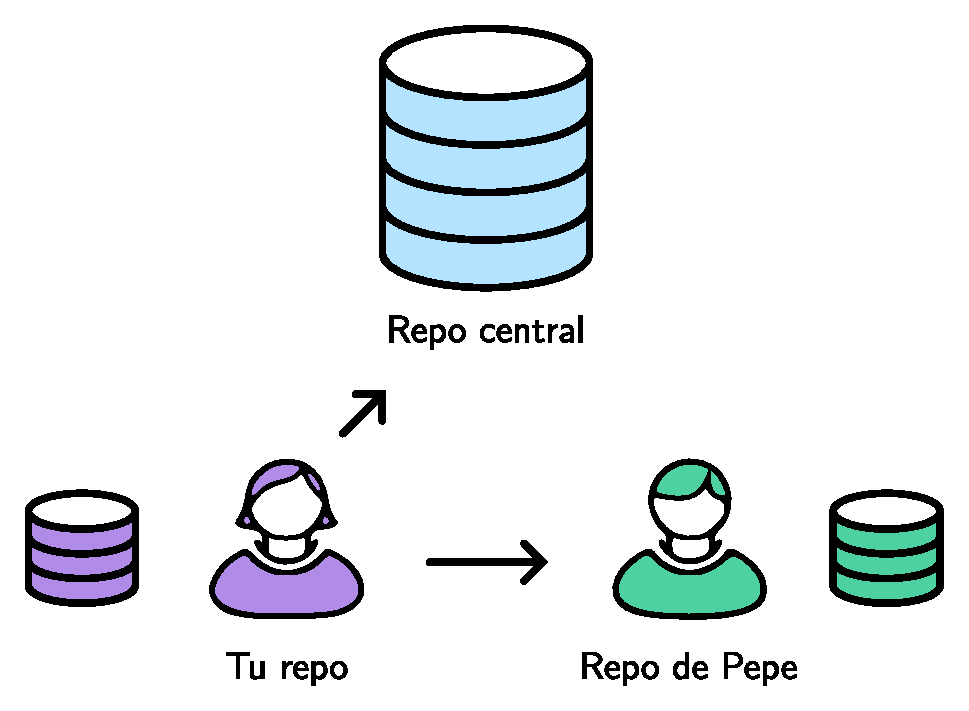
\includegraphics[height=1.5in]{images/repo-remoto.pdf}
        \end{center}
    \end{figure}

    Colaborar con otros implica gestionar estos repositorios remotos, y mandar (\textbf{push}) y recibir (\textbf{pull})
    datos de ellos cuando necesites compartir cambios.

\end{frame}

\begin{frame}{Usando Git online}
\begin{block}{Git server as a service}
    Para subir nuestros proyectos a Internet, ya sea para colaborar con otras personas o para compartir nuestro código, podemos usar un servicio de servidor web de Git.

    Los más conocidos son Github, Bitbucket y Gitlab. 
    \end{block}
    \begin{center}
        
\includegraphics[width=4in]{images/gitlab-logo-100.png}
    \end{center}

    También es posible hostear tu propia instancia de Git, por ejemplo \href{https://git.exactas.uba.ar/}{git.exactas.uba.ar}.

    Hay otros proyectos que comparten los \textit{commits} por mail, por ejemplo.
    % si hay una fotito de esto puede quedar bueno
\end{frame}

\begin{frame}[fragile]{Configuraciones iniciales 1/3}

    \begin{block}{Tu identidad}
        Es importante establecer nuestro \textbf{nombre y email} en nuestro repositorio, ya que estos van a ir asociados con los cambios que hagamos:

        \vspace{0.5em}

        \texttt{git config --global user.name "Guybrush Threepwood"}

        \texttt{git config --global user.email guybrush@example.com}

    También se puede omitir el flag \texttt{--global} para que las credenciales apliquen solo al repositorio en el que estamos trabajando.
        \end{block}
\end{frame}
\begin{frame}[fragile]{Configuraciones iniciales 2/3}

	\begin{block}{Clave SSH}
		Para poder trabajar cómodamente con repositorios Git que estén en Internet (GitHub, Bitbucket, GitLab, etc.), podemos configurar una \textbf{clave SSH} que nos identifique con el servidor que estemos usando. De esta manera, puede reconocer desde que usuario vienen los pedidos (para revisar permisos, etc...).

        %De esta manera, cuando tengamos un repositorio en Gitlab vamos a poder conectarlo con nuestro local.
	\end{block}
\end{frame}

\begin{frame}{Configuraciones iniciales 2/3}
  \begin{block}{Creando una clave nueva}
		Abrimos la terminal y ejecutamos \textit{cd \textasciitilde/.ssh} y luego \textit{ssh-keygen -f taller-git}. Le damos \textit{Enter} a todo. También podemos elegir asignarle una contraseña (aconsejable para compus compartidas).
	\end{block}
  \pause
  \begin{block}{Subiendo la clave a GitLab}
		\begin{itemize}
		\item En la terminal, ejecutamos \textit{cat taller-git.pub} y copiamos todo lo que aparezca.
      \item Abrimos GitLab, vamos a Profile Settings, SSH Keys.
      \item Pegamos lo que tenemos copiado en el campo \textit{Key}.
      \item Ponemos para que expire mañana y le damos al boton \textit{Add key}.
		\end{itemize}
	\end{block}
\end{frame}

\begin{frame}[t]{Vinculando un repositorio remoto}
    \begin{comando}
        git remote
    \end{comando}

    \vspace{0.5em}
    \pause
    \begin{block}{Ver los repositorios remotos asociados}
        Ejecutamos \texttt{git remote -v}. Si no hay ningun output, es que el repo no tiene ningún remote. Es decir, no apunta a ningún otro repo fuera del local.
    \end{block}

    \pause
    \begin{block}{Agregar un repositorio remoto}
        Ejecutamos \texttt{git remote add origin [URL]}. %chequear esto si funciona
    \end{block}

    % mover el tutorial de ssh antes de esto
    \begin{ejercicio}{Ejercicio}
        Agréguenle un \textit{remote} a algún repo, por ejemplo el de la clase pasada. Para esto tienen que crear un repositorio nuevo en GitLab y obtener su URL SSH.
    \end{ejercicio}
\end{frame}

\begin{frame}[t]{Enviando cambios}
    \begin{comando}
        git push
    \end{comando}

    \pause
    \begin{block}{}
        Para enviar los cambios \textbf{desde nuestro repositorio local a algún
        repositorio remoto}, ejecutamos \texttt{git push}.
    \end{block}

    \begin{ejercicio}{Ejercicio}
        Si tienen acceso al repo de la clase pasada, usen ese. Si no, pueden crear un nuevo usando los comandos que ya vimos. Asegúrense de hacer algún \textit{commit}. Luego hagan \textit{push}. 
    \end{ejercicio}
\end{frame}


\begin{frame}[t]{Obteniendo un repositorio Git}
        \begin{comando}
        git pull
    \end{comando}

    \begin{block}{}
        Para traer cambios \textbf{desde un repositorio remoto a nuestro repositorio local},
        ejecutamos \texttt{git pull}.
    \end{block}
    \pause
    \begin{comando}
        git clone
    \end{comando}

	\begin{block}{}
        Para obtener una \textbf{copia local} de un repositorio existente en algún servidor,
        utilizamos el comando \texttt{git clone [URL]}.

        En el caso de haber creado el repositorio con \textit{git init}, esto no es necesario. El comando \textit{clone} es como hacer \textit{init + remote add + pull}.
    \end{block}
\end{frame}

% \begin{frame}[t]{Y qué pasa si... ¡BOOM!}

%     \begin{block}{A veces hay conflictos}
%         \begin{itemize}
%             \item Supongamos que dos personas (\emoji{penguin} y \emoji{spouting-whale}) están trabajando en un mismo proyecto.
%                 Es decir, ambos tienen una \textit{copia} en su máquina.
%             \pause
%             \item Ahora imaginemos, por ejemplo, que \emoji{penguin} modifica la línea 23 del archivo \texttt{README}
%                 y confirma los cambios.
%             \pause
%             \item Sin saberlo, \emoji{spouting-whale} también modifica la línea 23 del archivo \texttt{README}, pero pone algo distinto y confirma dichos cambios.
%             \pause
%             \item ¿Qué va a pasar cuando quieran compartir lo que hicieron?\\ \only<6->{\textbf{Va a haber un conflicto},
%                 ya que dos personas modificaron de forma distinta la misma línea.}
%             \pause
%             \item ¿Qué va a hacer Git?\\ \only<7->{\textbf{Se va a quejar}. A alguno de los dos le va a tocar \textbf{incorporar a mano los cambios del otro}.}
%         \end{itemize}
%     \end{block}

% \end{frame}

% \begin{frame}[t]{Apagando el incendio}

%     \begin{block}{¿Cómo se ve un conflicto?}
%         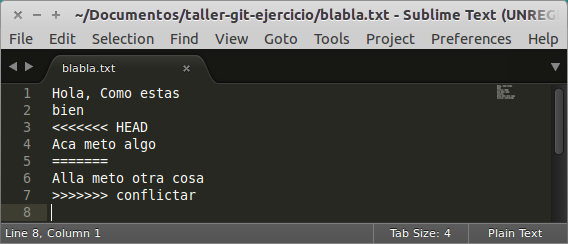
\includegraphics[height=1.0in]{images/conflicto.png}
%     \end{block}

%     \begin{block}{¿Qué hago?}
%         \begin{itemize}
%         \item Decido cómo tiene que quedar el archivo final (es decir, borro lo que quiera borrar manualmente).
%         \pause
%         \item Hago add.
% 		\pause
%         \item
%         Despues commit normalmente, con un mensaje como 'Merge'.
%         \end{itemize}
%     \end{block}

% \end{frame}

\begin{frame}[t]{¡A practicar!}

    \begin{ejercicio}{Ejercicio de a 2 máquinas (preferiblemente 2 personas): \emoji{christmas-tree} y \emoji{jack-o-lantern}}
        \begin{enumerate}\begin{small}
            \pause
            \item \emoji{christmas-tree}: crear un repositorio nuevo en \href{https://www.gitlab.com}{GitLab},
            y darle permiso a \emoji{jack-o-lantern} para hacer \textit{push}.
            \pause
            \item \emoji{christmas-tree} y \emoji{jack-o-lantern}: obtener una copia local del repositorio usando \textit{git clone}.

            \pause
            \item \emoji{christmas-tree}: 
            crear un archivo \textit{navidad.txt} con unas palabras acerca de la navidad.
            \item \emoji{jack-o-lantern}: crear un archivo \textit{halloween.txt} con unas palabras acerca de halloween.
            \pause
            \item \emoji{christmas-tree} y \emoji{jack-o-lantern}: hagan \textit{commits} con sus cambios respectivos.
            \pause
            \item \emoji{christmas-tree}: hacer \textit{push} con sus cambios.
            \pause
            \item \emoji{jack-o-lantern}: intentar hacer \textit{push} de los cambios al repositorio remoto. ¿Qué pasó?
            \pause
            \item \emoji{jack-o-lantern}: bajarse los cambios del repositorio remoto. ¿Anduvo?
            \pause
            \item \emoji{jack-o-lantern}: \textit{pushear} el resultado.
            \pause
            \item \emoji{christmas-tree}: bajarse los nuevos cambios.
        \end{small}\end{enumerate}
    \end{ejercicio}

\end{frame}

\begin{frame}{Visualizando los cambios 1/2}
\begin{center}
    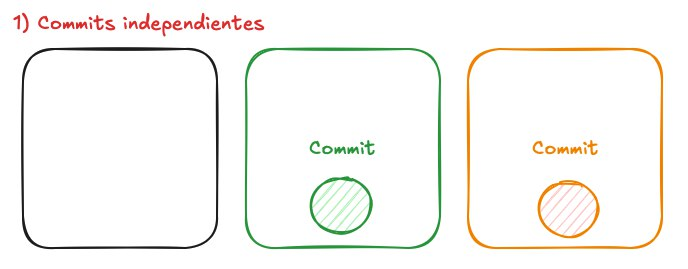
\includegraphics[width=2.5in]{images/merge1.jpg}
    \pause
    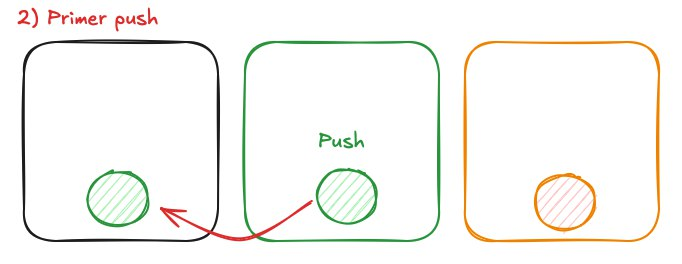
\includegraphics[width=2.5in]{images/merge2.jpg}
    \pause
    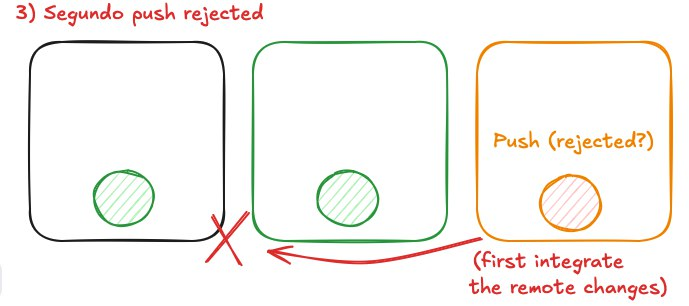
\includegraphics[width=2.5in]{images/merge3.jpg}
\end{center}
\end{frame}

\begin{frame}{Visualizando los cambios 2/2}
\begin{center}
    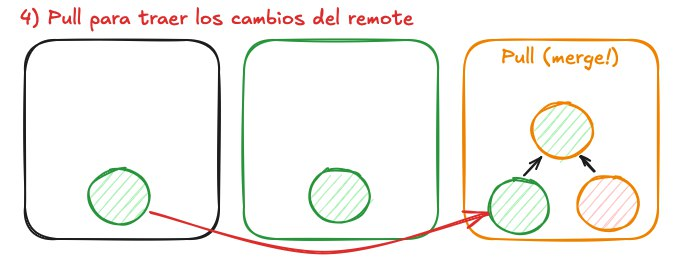
\includegraphics[width=2.5in]{images/merge4.jpg}
    \pause
    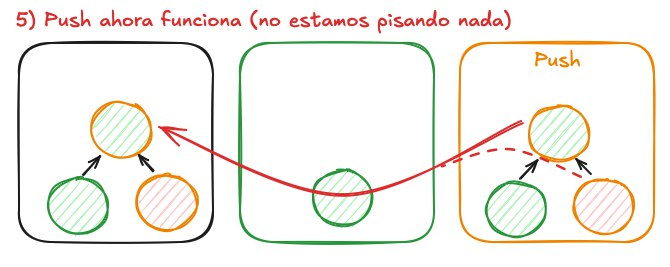
\includegraphics[width=2.5in]{images/merge5.jpg}
    \pause
    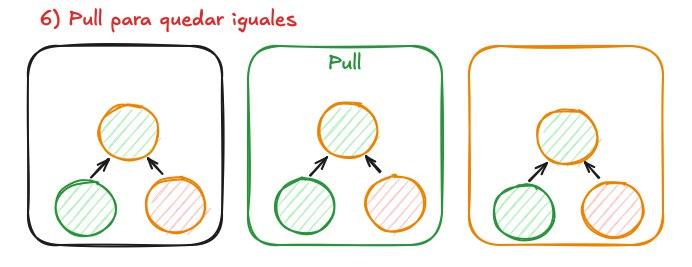
\includegraphics[width=2.5in]{images/merge6.jpg}
\end{center}

\end{frame}
